\documentclass[tikz,border=7pt]{standalone}
\usepackage{amsmath}
\usetikzlibrary{arrows.meta,positioning,fit}

\tikzset{
  comp/.style={draw,rectangle,minimum width=30mm,minimum height=13mm,align=center},
  port/.style={draw,circle,minimum size=5mm,inner sep=0pt},
  connect/.style={thick},
  flow/.style={-{Latex[length=2mm]},thick,dashed}
}

\begin{document}
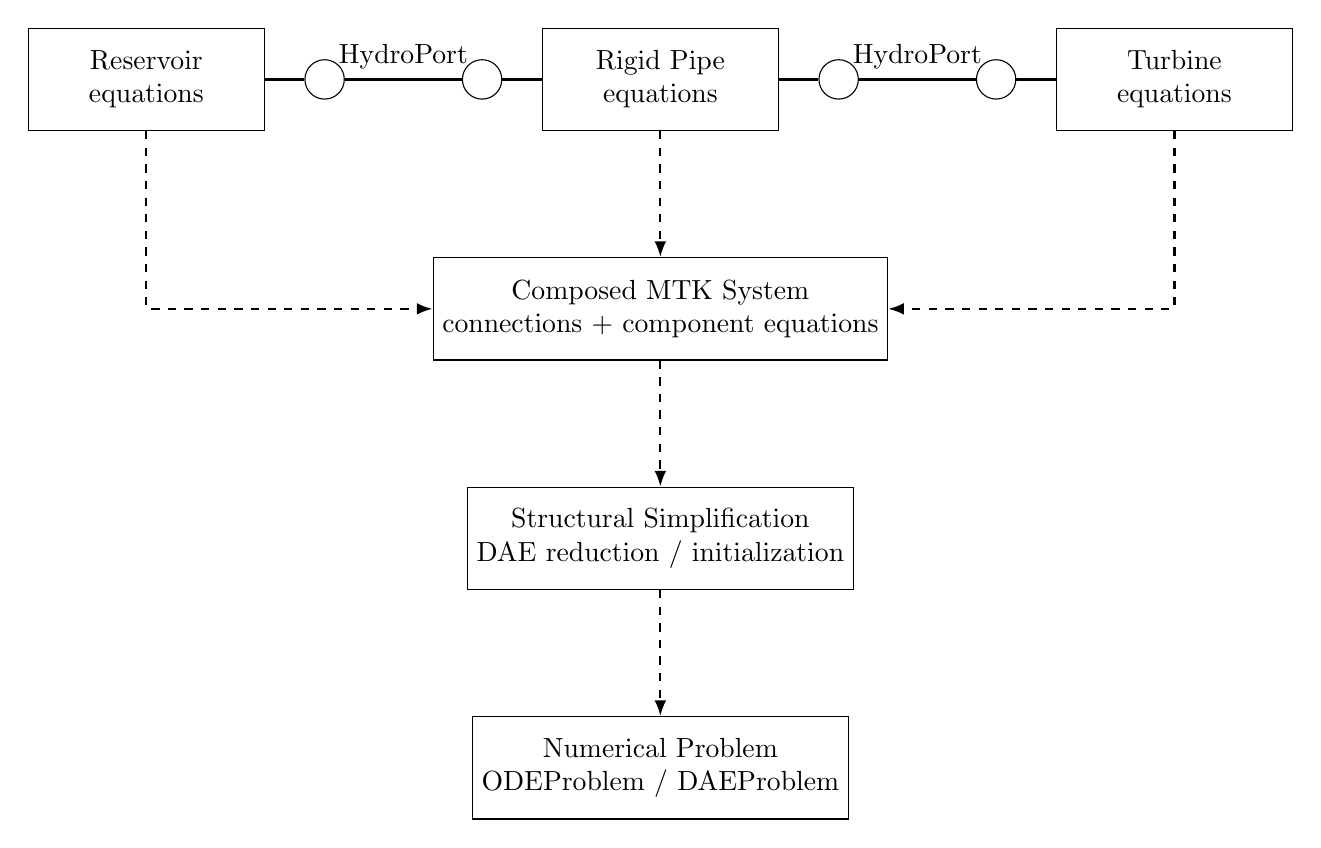
\begin{tikzpicture}[node distance=16mm and 22mm]

\node[comp] (res) {Reservoir\\equations};
\node[port,right=5mm of res] (p1) {};

\node[comp,right=25mm of p1] (pipe) {Rigid Pipe\\equations};
\node[port,left=5mm of pipe] (p2) {};
\node[port,right=5mm of pipe] (p3) {};

\node[comp,right=25mm of p3] (turb) {Turbine\\equations};
\node[port,left=5mm of turb] (p4) {};

\draw[connect] (res.east) -- (p1);
\draw[connect] (p1) -- node[above] {HydroPort} (p2);
\draw[connect] (p2) -- (pipe.west);
\draw[connect] (pipe.east) -- (p3);
\draw[connect] (p3) -- node[above] {HydroPort} (p4);
\draw[connect] (p4) -- (turb.west);

\node[below=16mm of pipe,comp] (sys) {Composed MTK System\\connections + component equations};
\node[below=16mm of sys,comp] (simp) {Structural Simplification\\DAE reduction / initialization};
\node[below=16mm of simp,comp] (prob) {Numerical Problem\\ODEProblem / DAEProblem};

\draw[flow] (res.south) |- (sys.west);
\draw[flow] (pipe.south) -- (sys.north);
\draw[flow] (turb.south) |- (sys.east);
\draw[flow] (sys) -- (simp);
\draw[flow] (simp) -- (prob);

\end{tikzpicture}
\end{document}
